\documentclass[10pt, letterpaper]{article}
% !TeX root =../main.tex
% !TeX spellcheck = en_US

\usepackage[in]{fullpage}
\usepackage{hyperref}
\usepackage[utf8]{inputenc}
\usepackage[numbers]{natbib}
\usepackage{doi}
\usepackage[affil-it]{authblk}
\usepackage{xspace}
\usepackage{amssymb}
\usepackage{amsmath}
\allowdisplaybreaks
\usepackage[numbers]{natbib}
\usepackage[utf8]{inputenc}
\usepackage[T1]{fontenc}
\usepackage[USenglish ]{babel}
\usepackage{url}
\usepackage{enumerate}
\usepackage{paralist}
\usepackage{here}
\usepackage[textsize=footnotesize]{todonotes}
\usepackage{doi}
\usepackage{xspace}
\usepackage{lipsum}

\usepackage{multirow}
\usepackage{siunitx}
\sisetup{locale = US}
\DeclareSIUnit{\mph}{mph}


\usepackage{tikz}
\usepackage{xcolor}
\usetikzlibrary{shapes}

% !TeX root =../main.tex
% !TeX spellcheck = en_US

\xspaceaddexceptions{())]\}}
\newcommand{\VRPTW}{VRPTW\xspace}



\title{DRAFT \\
Bridge Capacities
}
%Finding the optimal fleet size and mix for
%grocery home delivery services
% \footnote{This work was supported by Lakeside Labs GmbH, Klagenfurt, Austria and funding from the European
% Regional Development Fund and the Carinthian Economic Promotion Fund (KWF) under grant 20214/31942/45906.}
% }

\author[1]{Christian Wankm\"uller}

\author[2] {Christian Truden}
\author[3]{Andreas Felsberger}
% \affil[1]{Department of Mathematics, Alpen-Adria-Universit\"at Klagenfurt, Klagenfurt, Austria.}
\affil[1,3]{Department of Operations Management and Logistics, Alpen-Adria-Universität Klagenfurt,
Klagenfurt, Austria}
\affil[2]{Lakeside Labs, Klagenfurt, Austria}



\begin{document}

\maketitle

\begin{abstract}
  % !TeX root =./main.tex
% !TeX spellcheck = en_US

The transportation of oversize and heavyweight cargoes (OHC) represents one of the most challenging processes in freight movement, frequently leading to time-consuming and costly road closures, traffic congestions and temporary adaptations of infrastructure. In recent years, OHC transportation is gaining massive momentum due to an increasing economic development, general technological progress, and the growing prevalence of large-scale facilities such as wind mills or power plants. Apart from cost and time-related factors, security and safety issues have top priority when undertaking OHC transports on the road. Planning such transports is a complex task due to a multitude of criteria that need to be evaluated before determining the final route. In addition to physical road characteristics, road turning radius and transport corridor widths, the maximum bridge carrying capacity is an important safety-relevant parameter that highly influences OHC transports. Critical incidents, such as the Genoa bridge collapse in 2018, are negative examples where poor maintenance coincides with planning insufficiencies and non-compliance to standards and regulations. In this study, we take up the problem of selecting the optimal route for OHC transports under certain restrictions. In doing so, we propose an integer linear model with the objective to minimize road distance while considering maximum bridge carrying capacities. We test the model to balance cost, time and safety of OHC transportation using data of the Austrian highway network.

\end{abstract}
\noindent%
{\it Keywords: Attended Home Delivery, Fleet Size, Tactical Planning}


\section{Introduction}
\label{sec:intro}
  % !TeX root =./main.tex
% !TeX spellcheck = en_US


Over-weight load, i.e., vehicles loaded with more than 11 tons per axle,
are even harder to plan then over-size load. Over-sized load is limited
by road turning radius, transportation corridor width and road-side obstacles, such as traffic lights, power lines. Hence planning is dominated these local characteristics
and in-person inspection of the suggest route.

In contrast to that, the planning process for over-weight includes the consultation
of an civil engineer who must determine the allowable weight and speed to pass
complex building structures such as bridges.
This time consuming process must be repeated once the intended route is determined infeasible or changes for any other reason.
In an attempt to relieve some of this cumbersome workload from civil engineers,
we propose an mathematical optimization approach.

To this end, a mathematical model determines the optimal path between two
points within the road network while respecting the bridge capacity constraints.
This serves as an \textit{decision support system} for civil engineers.
Ultimately,  each route must be must be approved by a civil engineer  in terms of
bridge capacities and other structural limitations.

Under the assumption that the model generates feasible routes,
we conduct a study that compares several (possibly conflicting) objectives.
Therefore, we consider different types of vehicles and different loads.

Possible objective are:
\begin{itemize}
  \item Shortest Path (classic).

  \item Minimal wear of infrastructure. Reducing the wear induced by over-weight transports
  minimizes maintenance costs, extends lifetime of the building structures, and
  improves safety (Genoa bridge collapse in 2018).

  \item Minimize the number of different road operators and municipalities the path
  traverses. In that sense, the process of getting official approval of the
  path should be simplified.
\end{itemize}

\section{Related Work}



\subsection{Morandi Bridge Colapse}

\cite{Morgese.2020}
\cite{MorandiNYTimes}


\section{Commercial Solutions}

\subsection{HERE}
\url{https://www.here.com/}

\subsection{Bentley Superload Routing}
\url{https://www.bentley.com/en/products/product-line/asset-performance/superload-routing}



\section{Road Network}

We consider the higher level road network, i.e., A, S, L, B.
and we vertices of the matrix crossing points of the roads.
the edges are the road section between those points, for which we
consider the distance the length of the bridges and their capacity constraints (and the lowest encountered bridge capacity).
This way we can, answer questions concerning transports between those vertices.

\begin{figure}
 \centering
  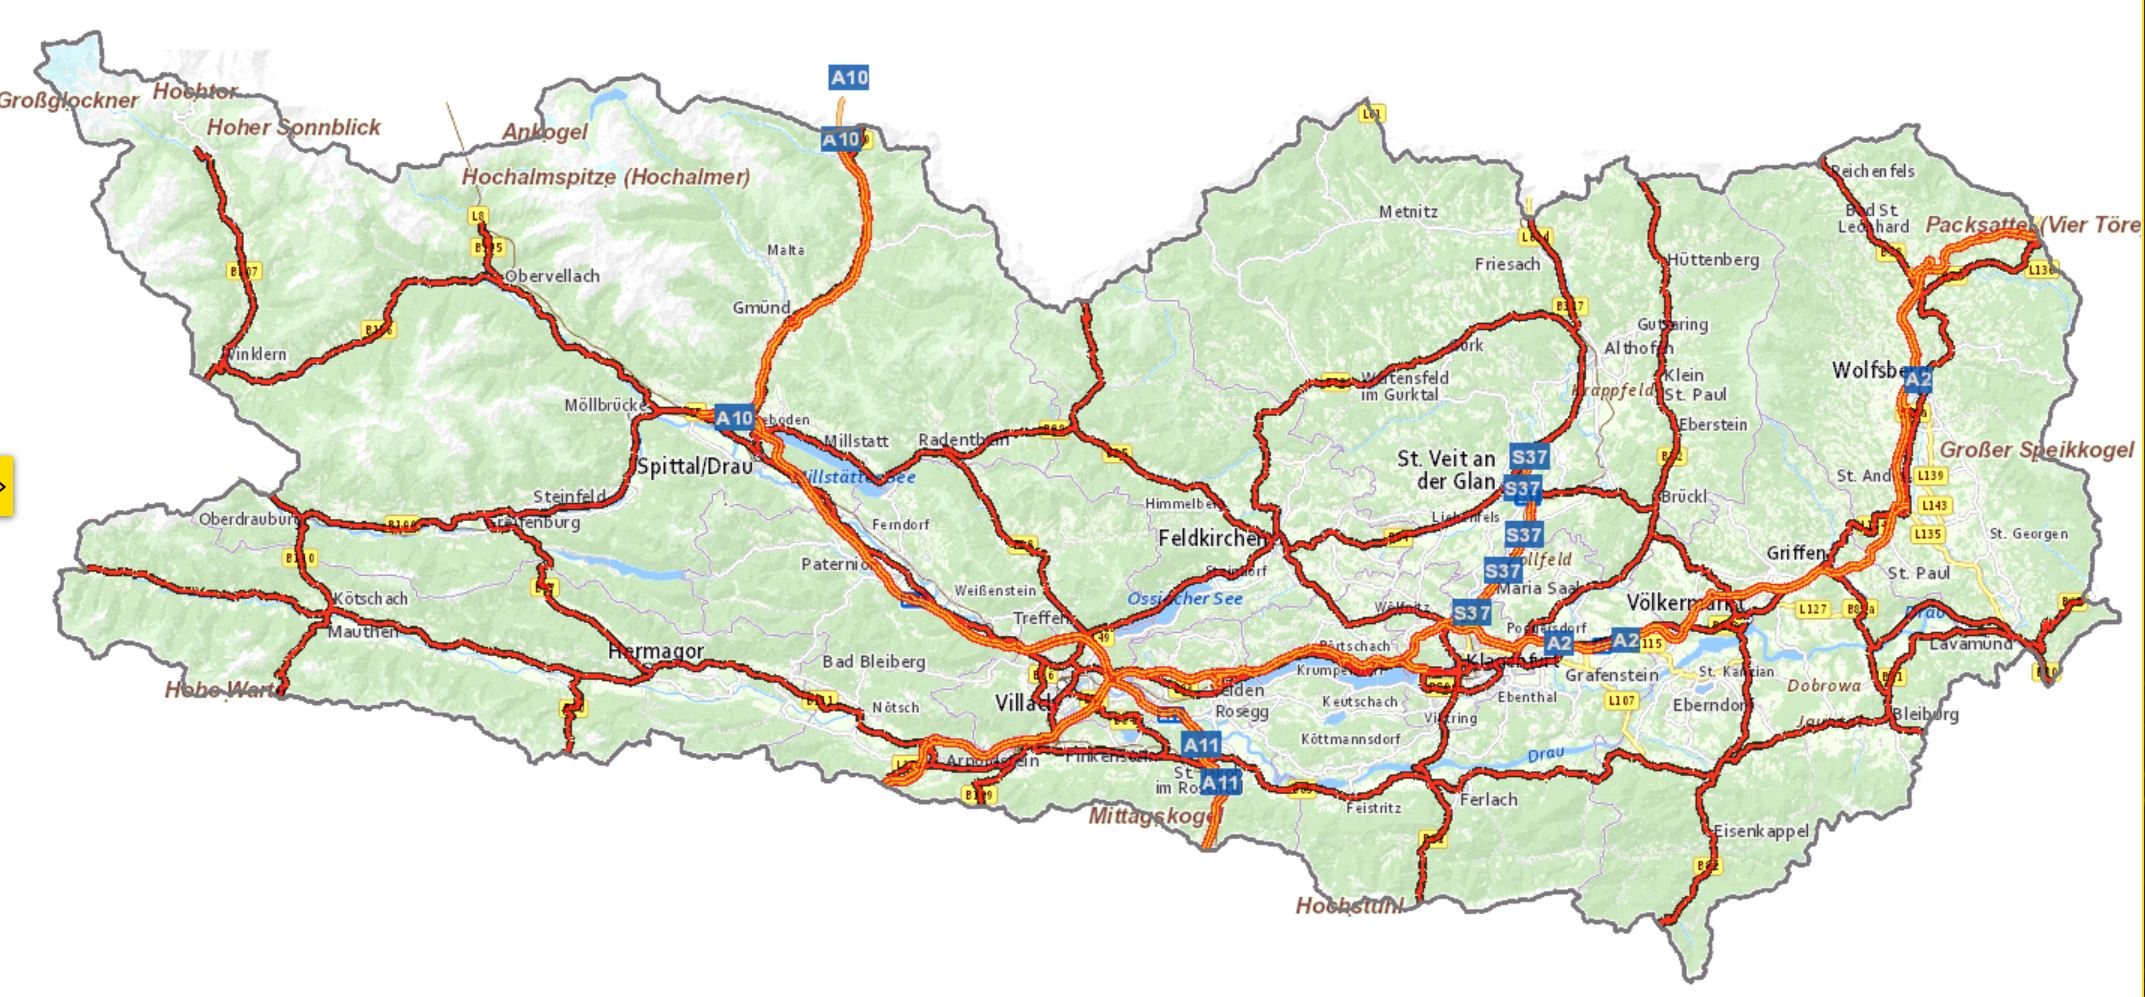
\includegraphics[width=0.9\textwidth]{map.jpg}
  \caption{Overview of the higher level road network in Carinthia.}
  \label{fig:higher level}
\end{figure}



\section{Related Work}\label{sec:intro}
%
% !TeX root =./main.tex
% !TeX spellcheck = en_US

Increasing economic development, general technological progress, and the growing prevalence of large-scale facilities, such as wind mills or power plants, increase the demand for OHC transports.
Frequently, these transport processes are executed within the road network. This is because roads exhibit a high geographical coverage and thus, provide a certain amount of flexibility and cost saving potential, as goods can often be delivered directly without any time-consuming handling or transshipment efforts being required. However, taking into account the complexity of road transportation as well as the potential damage caused to pavements and bridges, OHC route selection is a highly challenging task \cite{Bazaras.2013, xu2001methodology, sivilevicius2007dynamics, fiorillo2016minimizing}. Yet, selection of an optimal route based on reasonable route planning methods greatly improves the efficiency of OHC transports \cite{meng2015optimized}.
Therefore, optimal route selection in the field of road-related OHC has recently become a topic of considerable relevance \cite{geisberger2011efficient, yan2018optimal}.
\par
This paper is building upon past research on OHC routing. In the literature, a wide range of different approaches to this issue are presented. Fu and Hag-Elsafi \cite{fu2000vehicular}, for example, address the overload monitoring and permitting procedure. In doing so, reliability models for assessing bridge safety are described. Moreover, permit-load factors for monitoring purposes are proposed. Ghosn, in turn, focuses on truck weight regulations and the corresponding bridge safety levels using reliability indices \cite{ghosn2000development}. Vigh and Kollár, again, elaborate on methods that take into account different bridge structures as well as vehicle and loading characteristics in the permitting process \cite{vigh2006approximate, vigh2007routing}
\par
One particular method for optimal route selection is the integration and processing of all available data concerning the road network in a Geographic Information System (GIS) \cite{durham2002gis}.
According to Datla et al. \cite{datla2004gis}, a GIS facilitates identification of shortest paths, while taking into account characteristics and attributes of the road network as well as the involved transport vehicles, provided that data are available and up-to-date. Relevant parameters, such as vehicles' load, height, width, weight, and weight distribution, are considered to take into account restrictions, ensuring safety, and preventing damage to infrastructure elements such as bridges \cite{ecmt2006improving, vaitkus2016effect, kombe2017modelling, pauer2017development}. According to Adams et al. \cite{adams2002enterprise}, a GIS-based system also facilitates the automation of the permission process by considering spatial and temporal constraints during the path-finding process, given that the respective systems for routing and authorization purposes are well integrated. However, the authors also emphasize the difficulty of aligning enterprise databases of bridges and highways with the requirements of GIS-based permitting systems, which is frequently resulting in severe data management problems.
\par
According to Bazaras et al. \cite{Bazaras.2013}, safety, security, and reliability are indeed three very important aspects that have to be considered to increase the overall quality of transport processes. Therefore, apart from regular driving training and state-of-the-art equipment, detailed risk evaluation is regarded to be a key issue in terms of OHC routing. The authors also underline that a fuzzy multi-criteria decision making tool is beneficial in the course of route selection, as it allows taking into account the variety of influencing factors. Apart from road quality, turning radius, corridor widths and heights, bridge carrying capacities, reloading and storing opportunities, regular traffic intensity on route segments, and seasonal specialties, a multi-criteria system might also include an assessment of required road texture improvements and other structural adaptations or changes.
\par
In summary, the respective literature does not take adequate account of bridge carrying capacities as an important influencing factor for OHC route selection. We assume the underlying reason being a general lack of data and insufficient data quality on exact bridge locations and carrying capacities.



% \begin{itemize}
%
%   \item Commercial Solutions
%
%   \item HERE
%   \url{https://www.here.com/}
%   \item PRISMA
%   \url{https://www.prisma-solutions.com/}
%
%   \item Bentley Superload Routing
%   \url{https://www.bentley.com/en/products/product-line/asset-performance/superload-routing}
%
% \end{itemize}



% \section{Conclusion}
% \label{sec:concl}
% \input{x_conclusion}

\small
\bibliography{bibliography}
\bibliographystyle{abbrvnat}


\end{document}
